\chapter{Einleitung}
\label{Einleitung}

Das Pflichtpraktikum im sechsten Semester des Studiengangs \textbf{Informationstechnik und Systemmanagement} welches in Kooperation mit der \textbf{Robert Bosch AG} durchgeführt wurde fand im Zeitraum vom 08.02.2016 bis 30.04.2016 statt. In diesem Zeitraum wurden ca. 460 Stunden in die Arbeit des zugeteilten Projektes gesteckt.\\\\
Die Firma Bosch hat ihren Hauptsitz in der Boschstraße 7 in Hallein, wo der Werkteil 1 beheimatet ist. Ein zweiter Teil des Betriebes, der Werkteil 2 ist in die Gemeinde Rif ausgelagert.  Die Mitarbeiterzahl des Betriebes liegt bei ungefähr 1100 für beide Werkteile zusammen.\\
Im Werk 1 werden Komponenten für den Large Engine Bereich (Schifffahrt, Eisenbahn, Minenfahrzeuge) produziert. Dies erstreckt sich von den sogenannten \textit{Injektoren} bis hin zu kompletten Pumpensystemen für die unterschiedlichsten Motorentypen. Ebenso ist im Werkteil 1 der Musterbau, die Forschung und Entwicklung, das Qualitätsmanagement sowie der Versand beheimatet. \\
Der Werkteil 2 befasst sich mit der Produktion der DENOX Komponenten. Diese werden zur Abgasnachbehandlung verwendet, indem Stickoxide aus den Abgasen entfernt werden.\\\\
Im Zuge des Praktikums konnte ein Einblick in die verschiedenen Abteilungen des Betriebes erlangt werden, da dies für die Aufgabenstellung des Projektes von Nöten war.



\chapter{Arbeitsumgebung}
\label{Arbeitsumgebung}
Die Arbeit im Zuge des Praktikums war auf verschiedene Bereiche aufgeteilt. Der Großteil der Arbeit erfolgte im Büro am Schreibtisch, wo die verschiedenen notwendigen Softwarekomponenten entwickelt wurden. Weiterhin fielen aber auch Arbeiten abseits des Projektes in den verschiedenen Produktionshallen im Werkteil 1 und Werkteil 2 an.\\
 Das Arbeiten in den angesprochenen Produktionsanlagen unterschied sich von der Arbeit am Schreibtisch dadurch, dass hier vor allem auf die Sicherheit geachtet werden musste. So war es Vorschrift, im Bereich der Produktionsanlagen Sicherheitsschuhe zu tragen. Bei den Arbeiten im Produktionsumfeld wurden z.B. Kartenlesevorrichtungen an neu angelieferte Maschinen zur Laserbeschriftung angebracht und in das Netzwerk eingebunden.\\
 Für die Arbeit im Büro, zur Softwareentwicklung für das zugewiesene Projekt, wurde mit folgenden Frameworks / Programmiersprachen gearbeitet.
 
 \begin{itemize}
 \item Python
 \item CSS
 \item HTML 5
 \item JavaScript
 \item PHP
 \item mySQL
 \item Bootstrap
 \item jQuery
\end{itemize}  
Diese waren nötig um mit den verschiedenen Schaltungen (siehe Abschnitt \ref{Prototyping}) die entsprechenden Daten mittels Sensoren auszulesen.


\chapter{Projektdurchführung}
\label{Projektdurchführung}
Das Projekt \glqq Möglichkeiten zur Einbindung von Single Board Computern (SBC) in ein bestehendes Fertigungsumfeld\grqq
wurde am Beginn des Praktikums genau definiert. Enthalten sollte dies, die möglichen Bereiche, sowie die Einsatzmöglichkeiten von SBCs in diesen. Speziell sollte auf die Bereiche Temperatur- und Vibrationsmonitoring eingegangen werden, da diese Bereiche auch für die Qualität in der Produktion wichtig sind. Auch sollte bei der Realisierung des Projektes der Kostenfaktor berücksichtigt werden. Dies bedeutete, dass Aufgaben, die ansonsten mit teuren Komponenten realisiert werden müssten anhand günstigerer Varianten mit dem fast identischen Ergebnis bewerkstelligt werden können. Weiterhin sollten verschiedene Prototypen realisiert und getestet werden, sowie Möglichkeiten zu Datenspeicherung und Visualisierung erarbeitet werden. 

\section{Literaturrecherche}
Um die theoretischen Grundlagen für ein erfolgreiches realisieren des Projektes zu gewährleisten, befassten sich die ersten zwei bis drei Wochen mit der Literaturrecherche und dem studieren dieser. Da es in diesem Bereich noch nicht allzu viel Erfahrungen gibt, war es etwas anspruchsvoller gute Quellen zu finden. Zwei der wichtigsten Quellen sind im Literaturverzeichnis aufgeführt \citep{Bussysteme_in_der_Praxis} \citep{Raspberri_Pi_Handbuch}. Die wichtigsten Themen bei der Recherche waren, einen Überblick über die mögliche Hardware von verschiedenen SBCs sowie verschiedenen Sensoren und deren Schnittstellen zu bekommen. Des weiteren wurde sich mit den verschieden Bussystemen zum Auslesen der verschiedenen Sensoren beschäftigt. Einige Beispiele hierfür waren der I$^2$C-, SPI-, 1-Wire- und CAN-Bus. Für diese Themen, lieferte Quelle \citep{Bussysteme_in_der_Praxis} sehr gute Informationen.


\section{Theoretische Planung}
\label{Theoretische Planung}
Nachdem die Literaturrecherche abgeschlossen war, wurde sich auf Planung der einzelnen Schaltungen für die nachfolgenden Prototypen konzentriert. Diese Schaltungen wurden anhand der Datenblätter der einzelnen Sensoren entworfen und mittels dem Programm \textit{Fritzing} gezeichnet. Es wurden in diesem Bereich der Planung drei verschiedene Schaltungen entworfen, die im folgenden kurz dargestellt sind\footnote{Einige Passagen dieses und des nächsten Abschnittes wurden aus der BA2 entnommen}.\newpage

\begin{figure}[!h] 
  \centering
     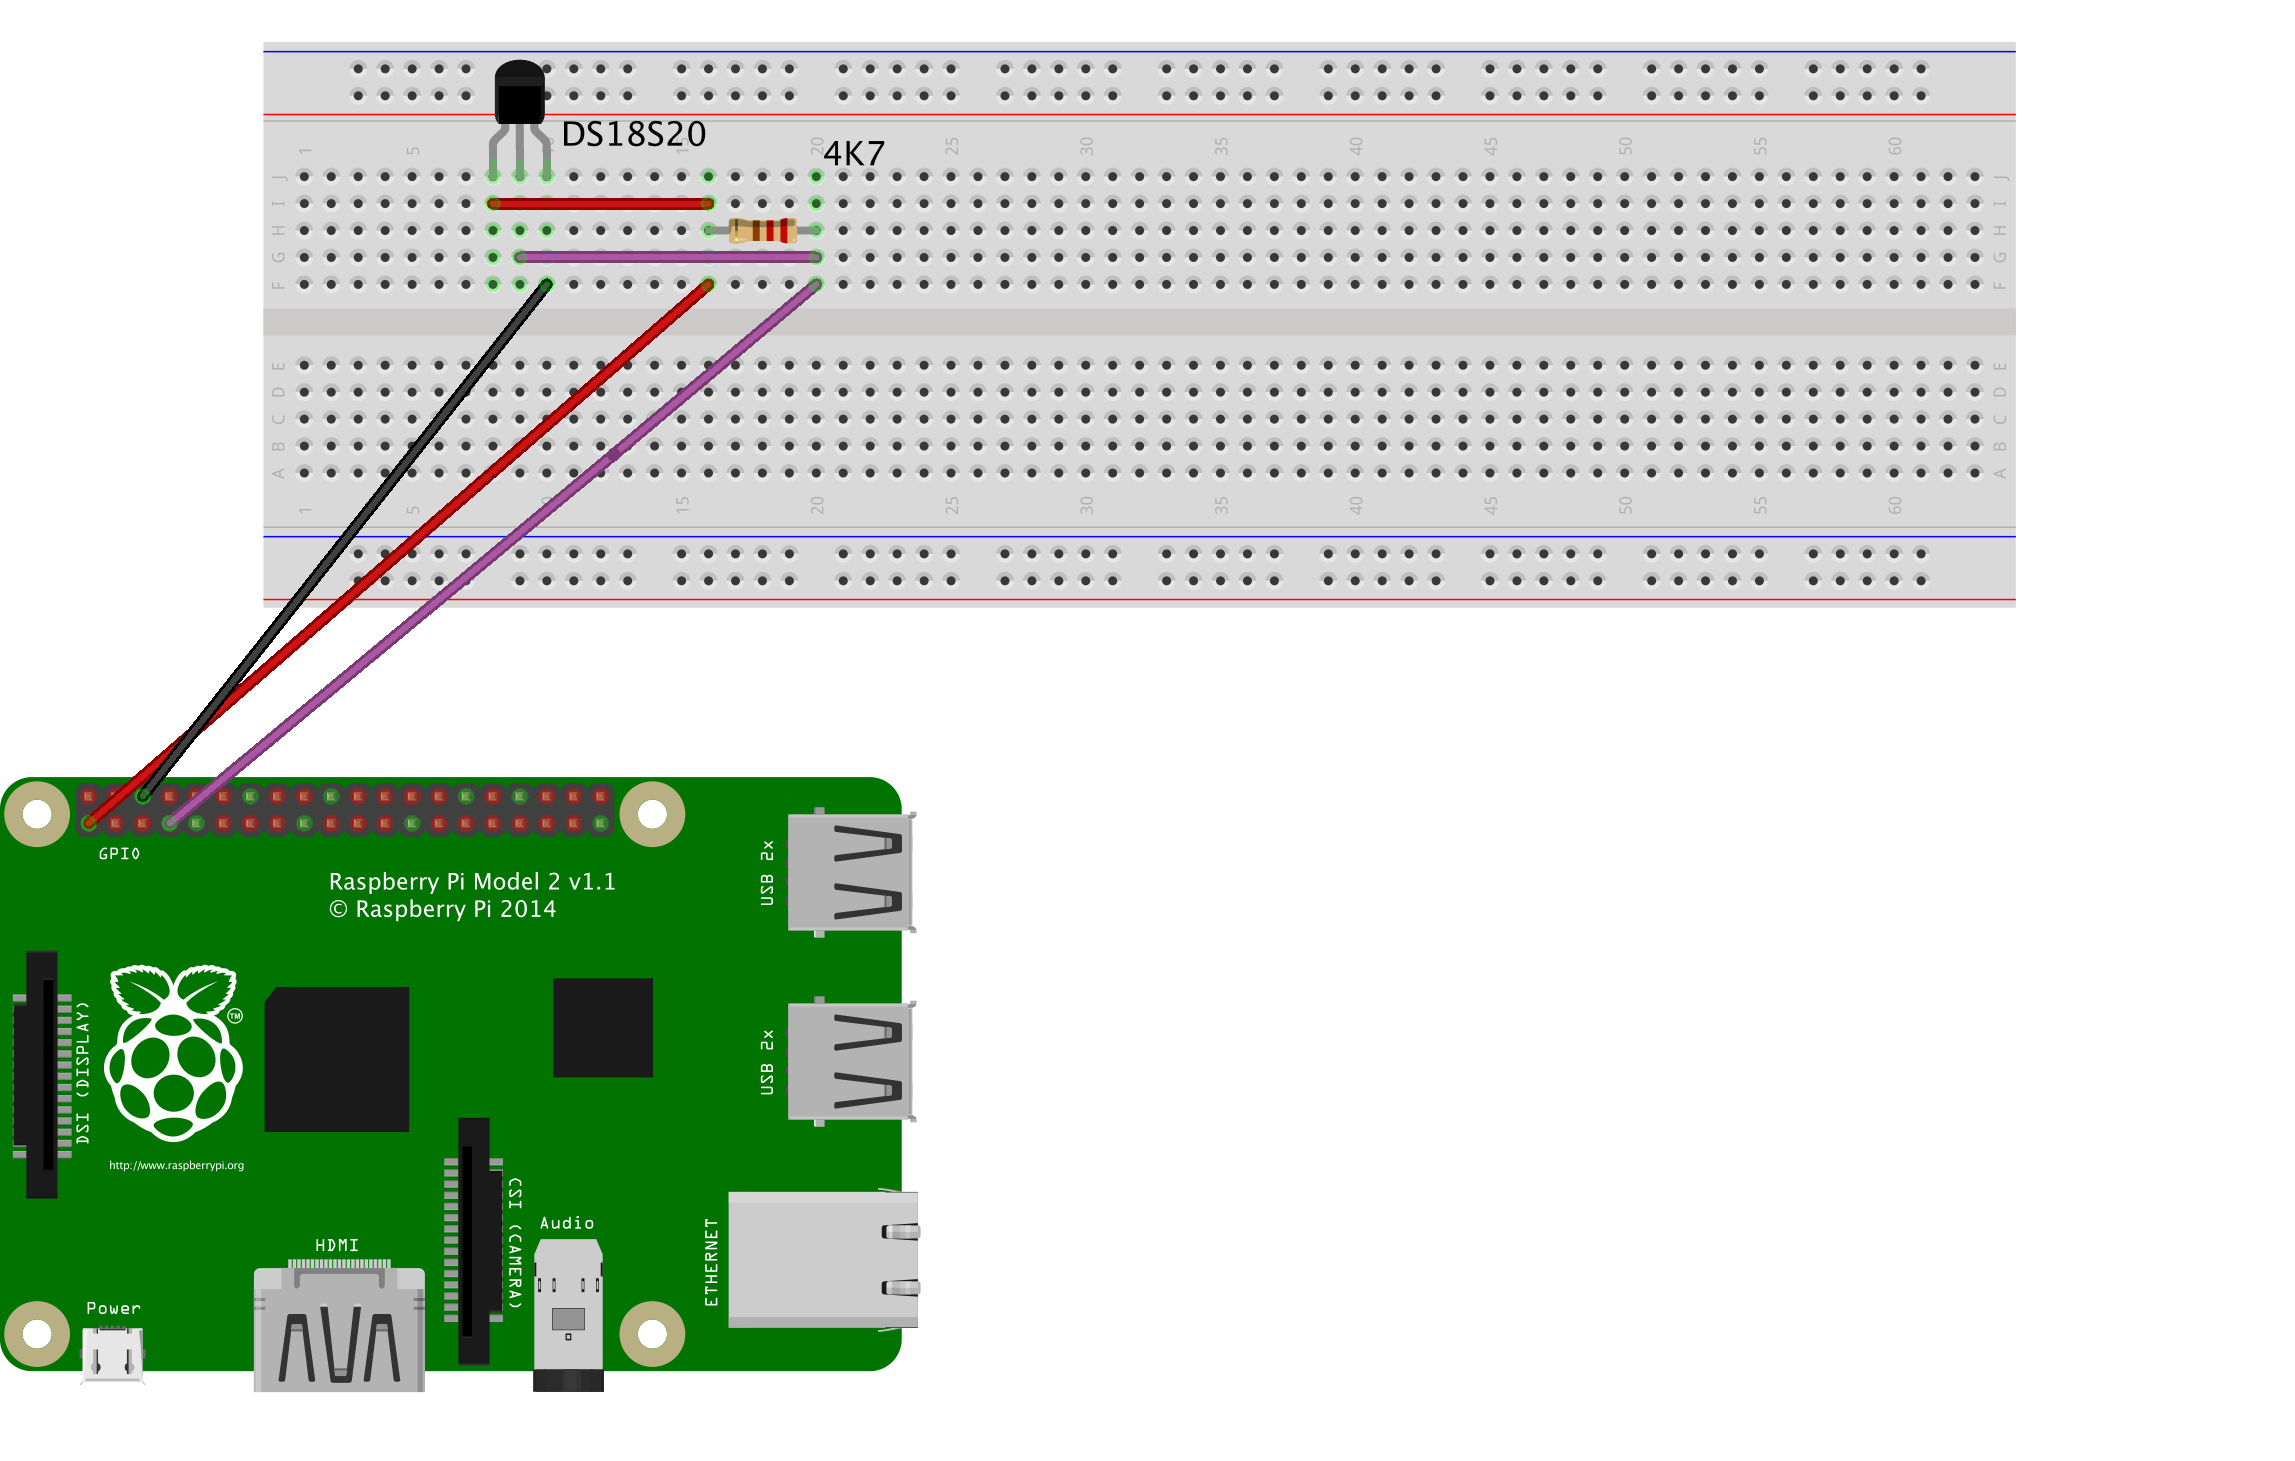
\includegraphics[scale=.4]{BilderAllgemein/Schaltung_DS18S20.png}
  \caption{Schaltung mit einem Temperatursensor}
  
\end{figure}

\begin{figure}[!h] 
  \centering
     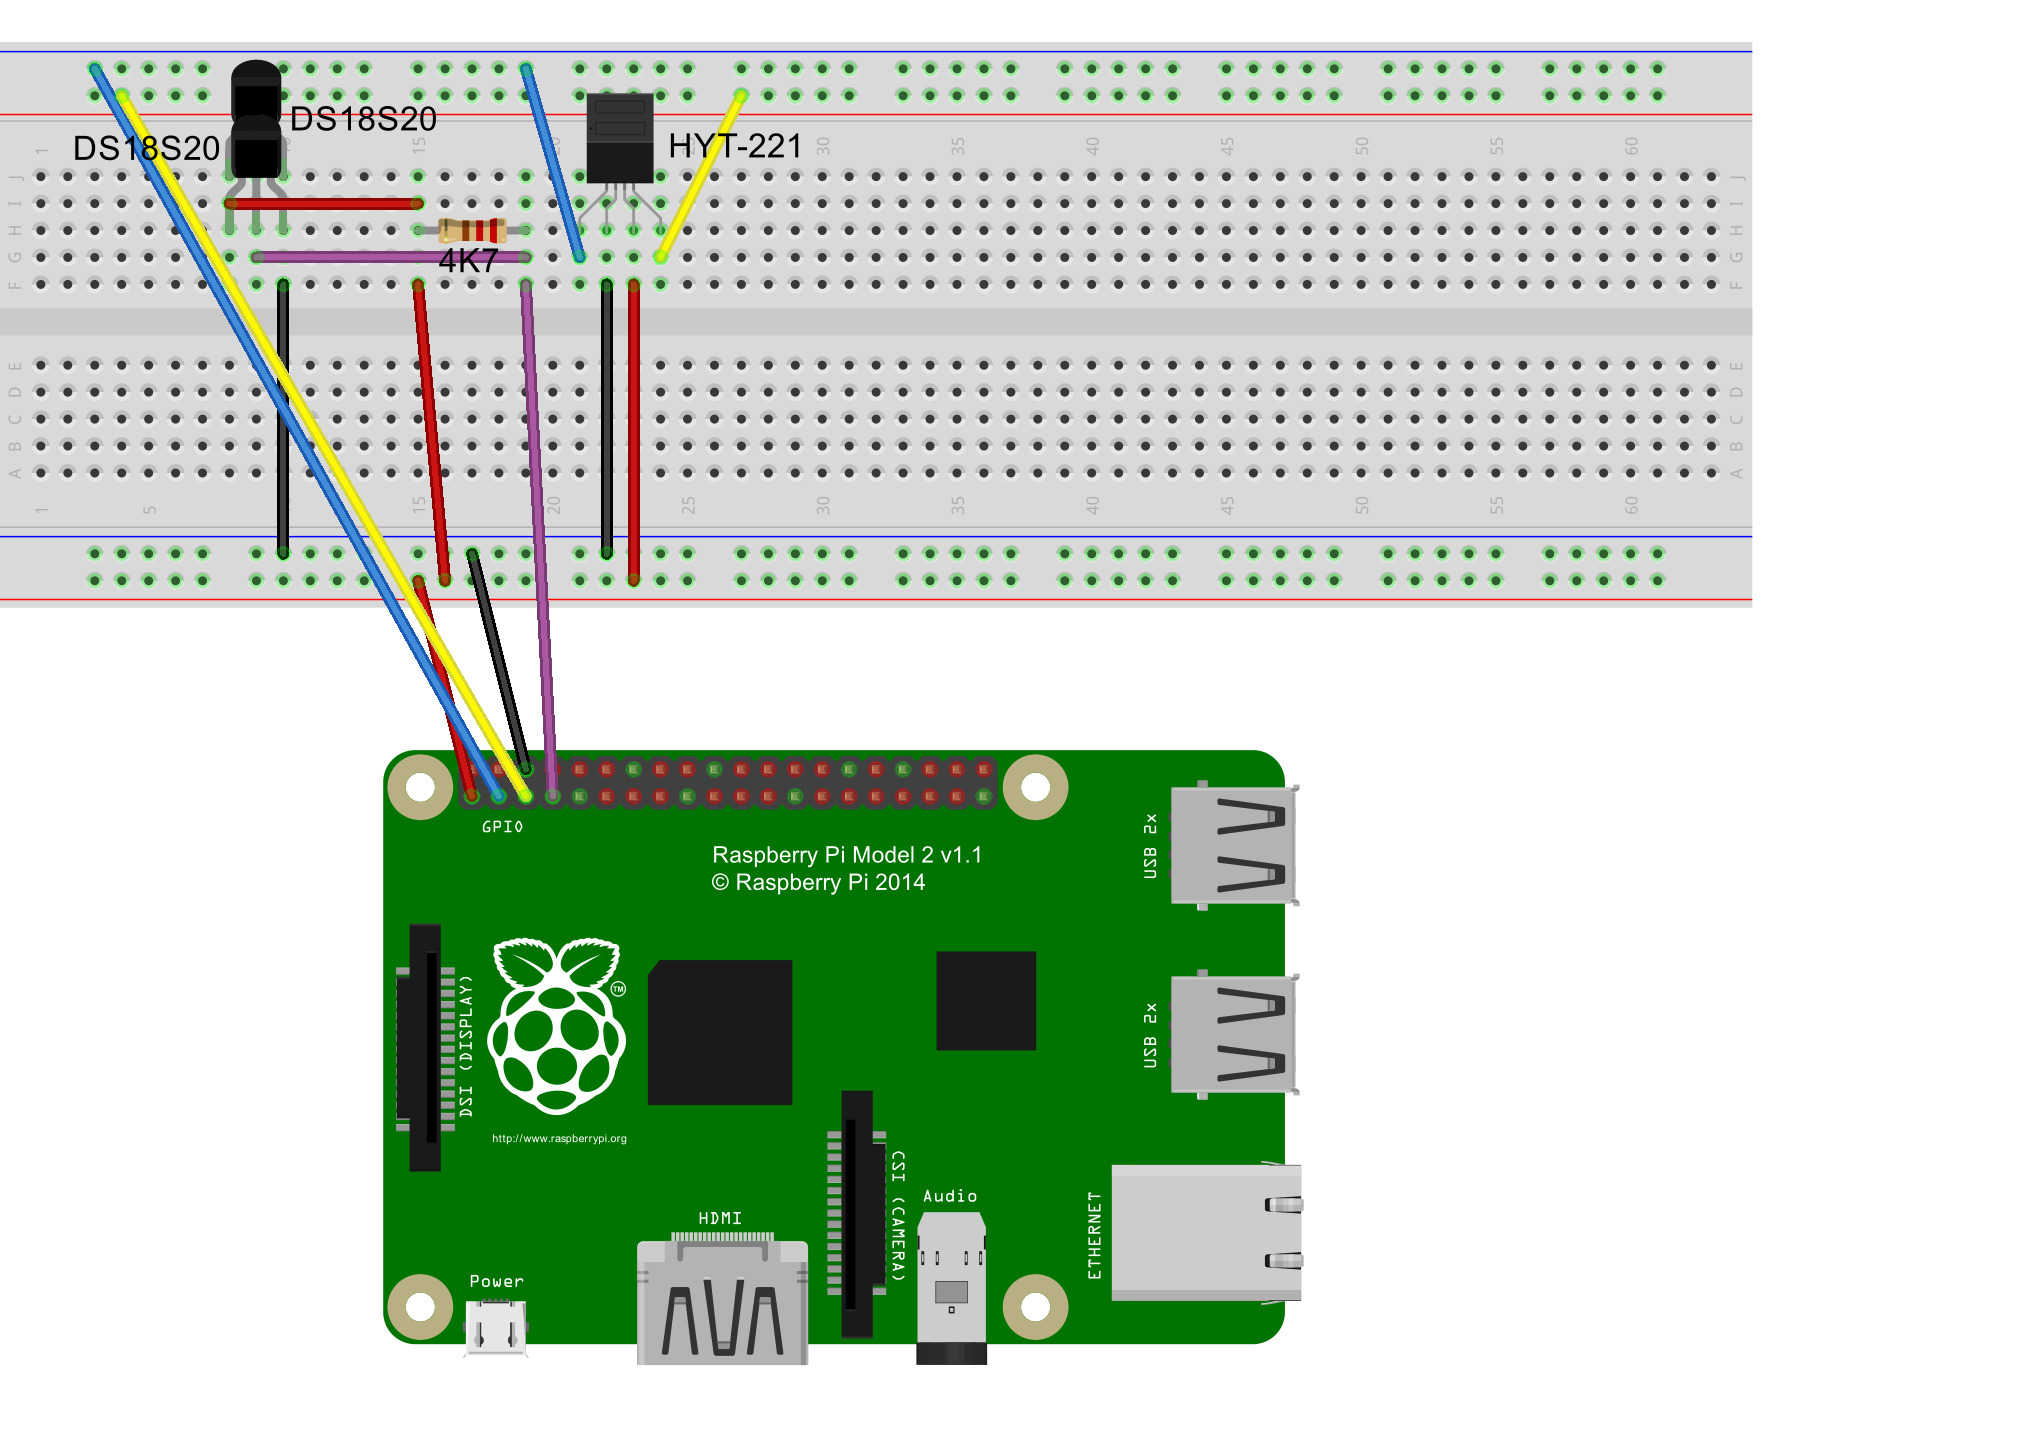
\includegraphics[scale=.4]{BilderAllgemein/Schaltung_HYT221.png}
  \caption{Schaltung mit drei Sensoren}

\end{figure}

\begin{figure}[!h] 
  \centering
     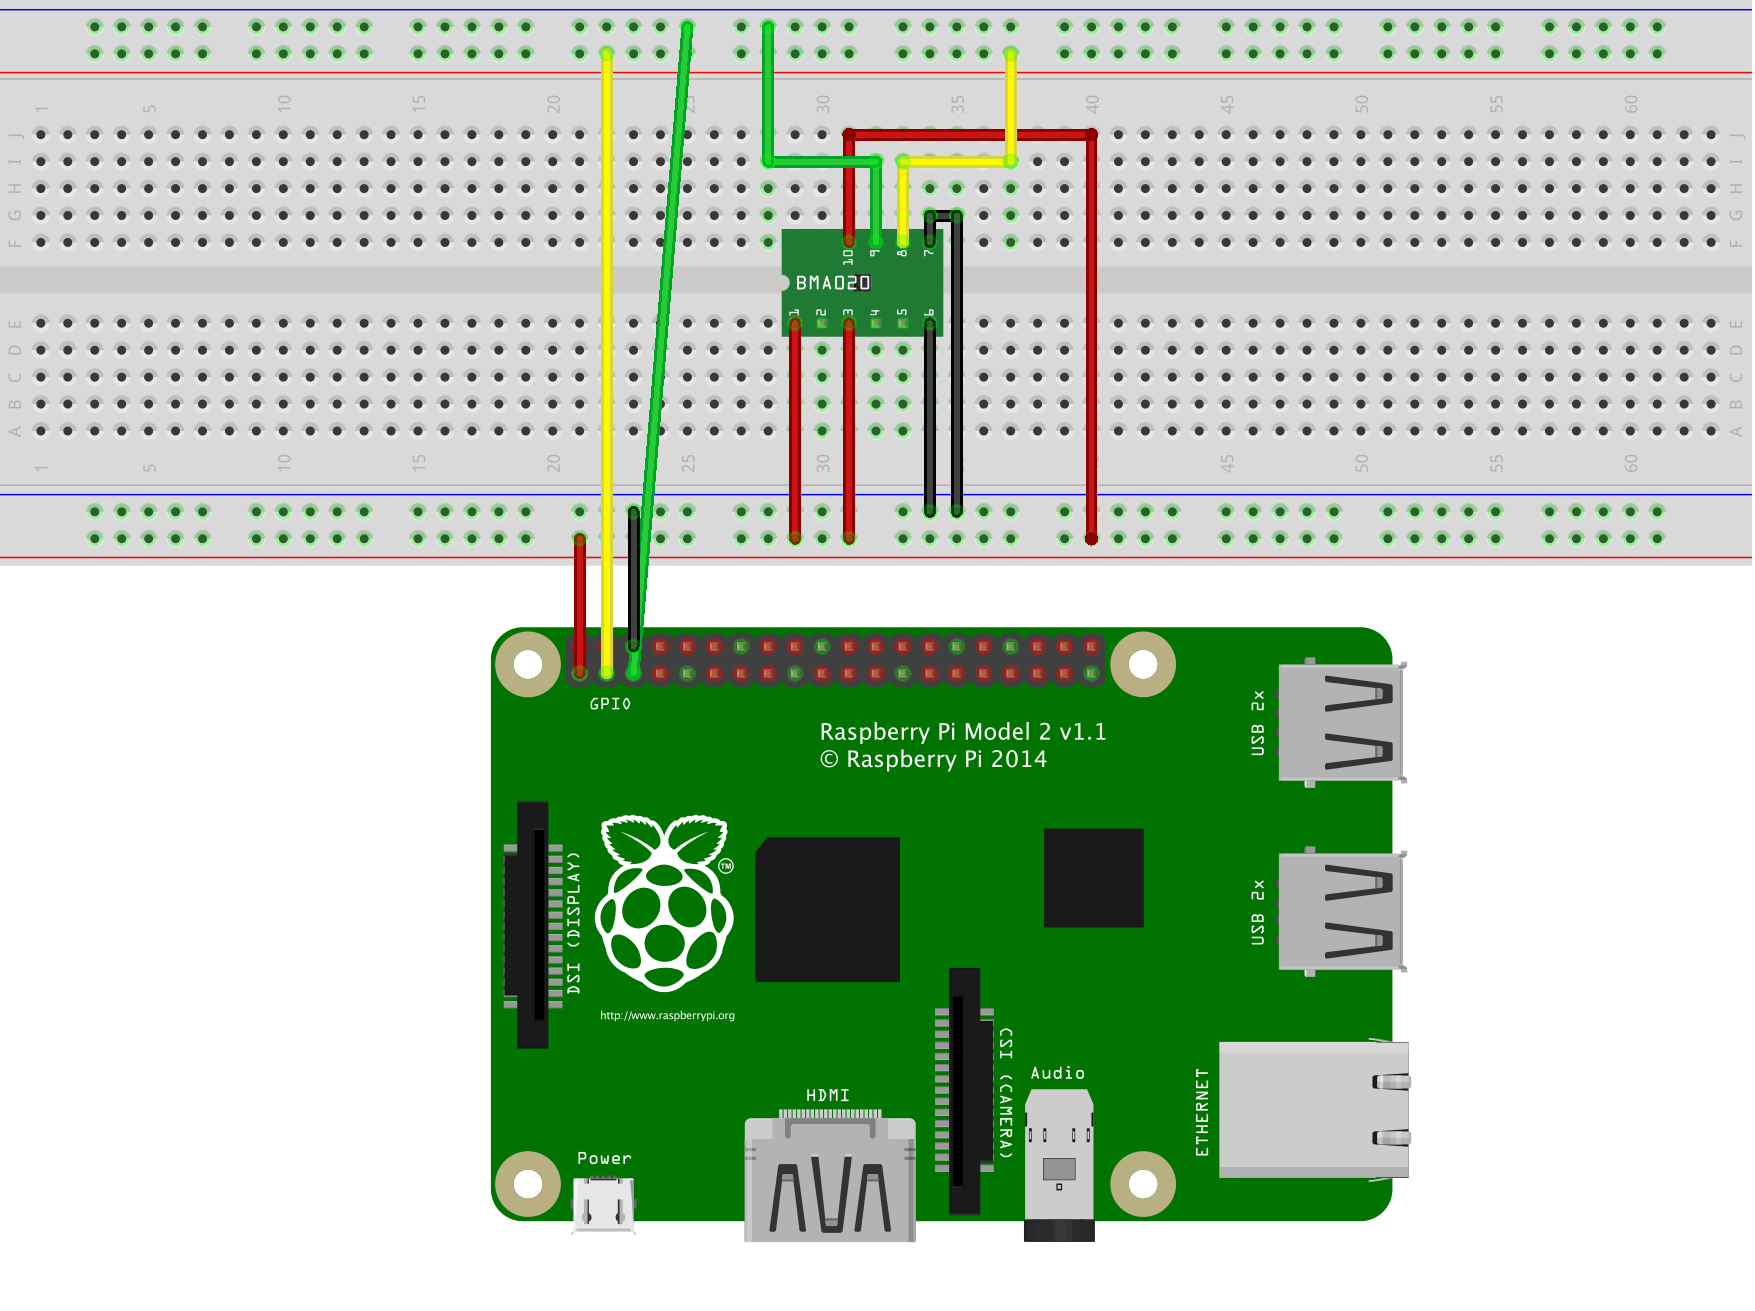
\includegraphics[scale=.4]{BilderAllgemein/Schaltung_Vib.png}
  \caption{Schaltung mit einem Vibrationssensor}
 
\end{figure}

Bei der theoretischen Planung der Schaltungen war es vor allem wichtig, die richtige Verkabelung der Sensoren mit dem dazugehörigen Pins des RPI sicherzustellen um einen möglichen Defekt eines Bauteils zu verhindern. Daher mussten die verschiedenen Datenblätter der einzelnen Komponenten sorgfältig studiert werden. Nachdem die Schaltungen erstellt waren, wurde sich der praktischen Durchführung dieser gewidmet.

\section{Prototyping}
\label{Prototyping}
Die praktischen Aufbauten und Erprobungen benötigten in diesem Projekt die meiste Zeit. Hier wurden die Schaltungen anhand der vorher entworfenen Schaltpläne praktische auf dem Steckbrett aufgebaut. Die verschiedenen Sensoren was für die einzelnen Versuche verwendet wurden, sind im Anschluss kurz aufgeführt.

\subsection*{DS18S20}
\label{subsection_DS18S20}
Der DS18S20  ist ein digitaler 1-Wire Temperatursensor, der eine Temperaturmessung mit 9\,Bit Auflösung ermöglicht. Dieser ist von der Firma \textit{Maxim Integrated} entwickelt worden.
Folgend werden die wichtigsten technischen Daten des DB18S20 aufgeführt.

\subsection*{HYT-221}
\label{subsection_HYT221}
Der HYT-221 ist ein Sensor zur Messung der Temperatur und Luftfeuchtigkeit. Er wurde von der Schweizer Firma IST für die Anwendung in den Bereichen Meteorologie, Industrielle Trocknungsprozesse, Medizinische Geräte, Luftfahrt und Extremsport entwickelt. Der Sensor kommuniziert über eine I$^2$C Schnittstelle und besitzt eine hohe Messgenauigkeit. 

\subsection*{BMA\,020}
\label{subsection_BMA020}
Der BMA\,020 ist ein von Bosch entwickelter Sensor, der die Beschleunigung in drei Richtungen (x-, y- und z-Achse) misst. Die Messdaten werden im Format eines 2er Komplements mit 10\,Bit ausgegeben. Als Schnittstellen stellt der BMA\,020 einen SPI- und I$^2$C Bus zur Verfügung.  

\subsection{Versuch 1}
Im ersten Schaltungsaufbau wurde ein DS18S20 verwendet um die Temperatur zu messen. Dieser wurde über den 1-Wire Bus betrieben. Auch kam hier das RRDtool zum Einsatz, welches Daten über einen bestimmten Zeitraum in eine Round Robin Datenbank speichert. Ein großer Vorteil diese Tools ist es, dass es wenig Speicherplatz für die Datenbank benötigt. Weiterhin kann mit Hilfe dieses Tools auch gleich eine grafische Aufbereitung erstellt werden. Der größte Zeitaufwand bei der Erstellung der Schaltung war, die verschiedenen Software Scripte zu erstellen, welche für das Auslesen, Speichern und Visualisieren der Daten benötigt wurden.

\subsection{Versuch 2}
Im zweiten Versuch wurde zum Aufbau aus Versuch 1 ein weiterer DS18S20 hinzugefügt und als dritter Sensor ein HYT-221, welcher zusätzlich noch die Luftfeuchtigkeit messen kann. Die Datenspeicherung und Visualisierung wurde gleich zum Versuch 1 durchgeführt. Weiterhin kam in diesem Versuch noch zusätzlich eine SQL Datenbank zur Speicherung der Messwerte zum Einsatz. Die für diesen Versuch benötigte Zeit war geringer als beim ersten Versuch, da einige Software wieder verwendet werden konnte oder ggf. nur ergänzt werden musste.

\subsection{Versuch 3}
Der dritte Versuch war von allen der anspruchsvollste, da hier die Änderung der Werte für den verwendeten Vibrationssensor BMA\;020 in nahezu Echtzeit dargestellt werden musste. Dies wurde über eine Darstellung mittels HTML Website und AJAX realisiert. Zur Datenspeicherung wurde hier eine SQL Datenbank verwendet, welche es ermöglicht, die gespeicherten Daten für eine spätere Verwendung in verschiedenen Formaten zu exportieren. Das Auslesen der Daten aus dem Sensor gestaltete sich hier schwieriger als bei den andern, da die Messwerte in verschiedenen Registern abgelegt waren und diese dementsprechend ausgelesen und zusammengesetzt werden mussten.

\vspace{1cm}
Bei der Arbeit an den praktischen Aufbauten wurde der Fortschritt der einzelnen Versuche in einem zwei wöchentlichen Rhythmus dem Betreuer und Arbeitskollegen präsentiert. Dies war für den Verlauf des Projektes positiv, da bei den Kollegen ein großes Interesse für dafür herrschte und das entsprechende Feedback sehr hilfreich war.


\chapter{Reflexion}
Zusammengefasst kann festgehalten werden, dass das Berufspraktikum eine sehr gut Sache war, da erste praktische Erfahrungen in den verschieden Bereichen gemacht werden konnten, welche für weitere Aufgaben sehr hilfreich sind. Auch war er sehr interessant, die Ablaufe und die Zusammenarbeit der einzelnen Abteilungen in einem großen Betrieb näher kennenzulernen.\\
Das Projekt selbst wurde als anspruchsvoll aber enorm interessant wahrgenommen. Ein großer Vorteil hier war, dass zwar bestimmte Vorgaben definiert wurden aber ansonsten die Richtung in die es sich entwickelte selbst bestimmt werden konnte. Dies wiederum förderte eine Menge Eigeninitiative und führte dazu, dass sich intensiv mit den verschiedensten Techniken bzw. Hardware auseinandergesetzt wurde. Durch diese breite Fächerung des benötigten Wissens, konnten die im Studium erlernten Kenntnisse in den verschiedensten Bereichen erweitert und gefestigt werden.